\documentclass[9pt, aspectratio=169]{beamer}
\beamertemplatenavigationsymbolsempty
\setbeamertemplate{caption}[numbered]
\linespread{1.25}

% header and footer
\newcommand{\pageauthor}{}
\setbeamertemplate{footline}[text line]{%
    \parbox{\linewidth}{\scriptsize\vspace*{-24pt}\pageauthor\hfill\insertsection\hfill\insertpagenumber/\inserttotalframenumber}}

% lists
\setbeamerfont{itemize/enumerate subbody}{size=\normalsize}
\setbeamertemplate{itemize subitem}{\normalsize\raise1.25pt\hbox{\donotcoloroutermaths$\blacktriangleright$}}

% figures
\usepackage{graphicx}
\graphicspath{ {./figures/} }

% maths
\usepackage{amsmath}
\usepackage{amssymb}
\usepackage{amsfonts}
\usepackage{mathtools}

% tables
\usepackage{booktabs}
\usepackage{algorithm}
\usepackage{algorithmic}
\usepackage{caption}
\makeatletter
\AtBeginEnvironment{algorithmic}{\small}
\makeatother

% bibliography
\usepackage[style=ieee]{biblatex}
\bibliography{refs.bib}
\renewcommand*{\bibfont}{\footnotesize}

%----------------------------------------------------------------------------------------
%	TITLE PAGE
%----------------------------------------------------------------------------------------

\title[Deterministic Policy Gradient]{{\normalsize Topics in Reinforcement Learning} \\ \vspace{0.5em} Paper Presentation: Deterministic Policy Gradient and Goal Relabelling}
\author{Group 7 \\ \vspace{0.5em} Himanshu Singh \and Vikaskumar Kalsariya}
\date{April 15, 2025}

\begin{document}

\begin{frame}
  \titlepage
\end{frame}

%----------------------------------------------------------------------------------------
%	TABLE OF CONTENTS
%----------------------------------------------------------------------------------------

\begin{frame}
  \frametitle{Table of Contents}
  \tableofcontents
\end{frame}

%----------------------------------------------------------------------------------------
%	SECTION 1: BACKGROUND & MOTIVATION
%----------------------------------------------------------------------------------------

\section{Background and Motivation}
\renewcommand{\pageauthor}{Himanshu Singh}

\begin{frame}
  \frametitle{Recap: Policy Gradients}
  \begin{itemize}
    \item Previous policy gradient methods (e.g., REINFORCE) primarily assumed stochastic policies.
    \item Stochastic policies inherently perform exploration by sampling actions.
    \item Resulting algorithms are often on-policy.
    \item Limitations of on-policy algorithms:
      \begin{itemize}
          \item Sample inefficiency (data used once).
          \item Exploration can be ``unguided'' and slow.
      \end{itemize}
  \end{itemize}

  \begin{alertblock}{The Challenge with Continuous Actions}
      In continuous action spaces, i.e. $a \in \mathbb{R}^m$, finding $\operatorname*{argmax}_a Q^{\mu_\theta}(s, a)$ (needed for Q-learning or greedy policy improvement) requires optimization at each step, which is often computationally expensive, especially with complex function approximators.
  \end{alertblock}
\end{frame}

\begin{frame}
  \frametitle{Alternative: Deterministic Policies}
    \begin{itemize}
        \item Consider a deterministic policy $\mu: \mathcal{S} \to \mathcal{A}$, parameterized by $\theta$:
        \begin{equation*}
        a = \mu_\theta(s)
        \end{equation*}
        \item \textbf{Advantage:} For a given state $s$, the action is fixed. No sampling needed for action selection.
        \item \textbf{Challenge:} How to ensure exploration? Deterministic policies don't explore naturally.
        \item \textbf{Solution:}
          \begin{itemize}
              \item Use an off-policy approach. Enables techniques like experience replay.
              \item Use a separate \textit{stochastic behavior policy} $b(a|s)$ for exploration during training (e.g., adding noise to $\mu_\theta(s)$).
          \end{itemize}
    \end{itemize}
\end{frame}

%----------------------------------------------------------------------------------------
%	SECTION 2: Deterministic Policy Gradient (DPG)
%----------------------------------------------------------------------------------------

\section{Deterministic Policy Gradient (DPG)}

\begin{frame}
  \frametitle{Deterministic Policy Gradient Theorem}
    \begin{theorem}[Deterministic Policy Gradient \cite{silver2014deterministic}]
        Let $J(\theta)$ be the performance objective (expected discounted return) for a deterministic policy $\mu_\theta(s)$. Assuming the MDP satisfies the regularity conditions of continuity and boundedness in all parameters and variables, the gradient of $J(\theta)$ is given by:
        \begin{align*}
        \nabla_\theta J(\theta) &= \mathbb{E}_{s \sim \rho^\mu} \left[ \nabla_\theta \mu_\theta(s) \nabla_a Q^{\mu_\theta}(s, a) |_{a=\mu_\theta(s)} \right]
        \end{align*}
    \end{theorem}

    \begin{itemize}
        \item \textbf{Proof Sketch:}
            \begin{itemize}
                \item Differentiate the value function to get a recursive equation.
                \item Unroll the above equation to get an infinite sum.
                \item Represent the objective in terms of probability of visiting a state and its value.
                \item Differentiate the objective and substitute the derivative of value function.
            \end{itemize}
    \end{itemize}
\end{frame}

\begin{frame}
  \frametitle{Exploration with DPG}
    \begin{itemize}
        \item Since the learned policy $\mu_\theta(s)$ is deterministic, exploration must be added \textit{externally}.
        \item \textbf{Standard Approach:} Add noise to the actor's output action during training.
        \begin{equation*}
        a_t = \mu_\theta(s_t) + \mathcal{N}_t
        \end{equation*}
        where $\mathcal{N}_t$ is a noise process.
        \item \textbf{Alternate Approach:} Ornstein-Uhlenbeck (OU) Process.
        \begin{itemize}
            \item Generates temporally correlated noise, suitable for physical control problems with inertia.
            \item Discrete-time update: $\nu_{k+1} = \lambda \nu_k + \sigma \epsilon_k$, where $\epsilon_k \sim \mathcal{N}(0, I)$.
            \item Parameters: $\lambda$ (mean reversion), $\sigma$ (volatility).
        \end{itemize}
        \item Learning is off-policy because the data is generated by $a_t \sim b(a|s_t)$, not $a_t = \mu_\theta(s_t)$.
    \end{itemize}
\end{frame}

\begin{frame}
  \frametitle{DPG Algorithm}
    \begin{algorithm}[H]
    \captionsetup{font=small}
    \caption{Deterministic Policy Gradient}
    \begin{algorithmic}[1]
    \REQUIRE Differentiable policy $\mu_\theta(s)$, action-value function $Q(s, u, w)$.
    \REQUIRE Step sizes $\alpha_\theta, \alpha_w$. Discount $\gamma$.
    \STATE Initialize actor parameters $\theta$, critic parameters $w$.
    \FOR {each episode}
        \STATE Initialize state $s_0$.
        \FOR {$k = 0, 1, \dots, T-1$}
            \STATE Select action $u_k = \mu_\theta(s_k) + \text{Noise}$ \COMMENT{Exploration}
            \STATE Execute $u_k$, observe reward $r_{k}$ and next state $s_{k+1}$.
            \STATE Choose next action for target: $u' = \mu(s_{k+1}, \theta)$ \COMMENT{Deterministic target action}
            \STATE Calculate TD Error: $\delta \leftarrow r_{k} + \gamma Q(s_{k+1}, u', w) - Q(s_k, u_k, w)$.
            \STATE Update Critic: $w \leftarrow w + \alpha_w \delta \nabla_w Q(s_k, u_k, w)$. \COMMENT{TD Learning}
            \STATE Update Actor: $\theta \leftarrow \theta + \alpha_\theta \nabla_\theta \mu_\theta(s_k) \nabla_u Q(s_k, u, w)|_{u=\mu_\theta(s_k)}$. \COMMENT{DPG Update}
        \ENDFOR
    \ENDFOR
    \end{algorithmic}
    \end{algorithm}
\end{frame}

%----------------------------------------------------------------------------------------
%	SECTION 3: Deep Deterministic Policy Gradient (DDPG)
%----------------------------------------------------------------------------------------

\section{Deep Deterministic Policy Gradient (DDPG)}

\begin{frame}
  \frametitle{Motivation: DPG + Deep Learning}
    \begin{itemize}
        \item DPG provides a policy gradient for deterministic policies, suitable for continuous actions.
        \item Deep Q-Networks (DQN) demonstrated success using deep neural networks for value function approximation in high-dimensional state spaces (e.g., pixels) \cite{mnih2013playingatarideepreinforcement}.
        \item \textbf{Goal:} Stable and efficient off-policy learning for continuous control in complex environments.
          \begin{itemize}
              \item Combine the DPG actor-critic approach with the techniques that stabilized DQN \cite{lillicrap2015continuous}.
              \item Use deep neural networks for both actor ($\mu_\theta(s)$) and critic ($Q(s, a, w)$).
              \item Adapt DQN's stabilization techniques: Experience Replay Buffer, Target Networks.
          \end{itemize}
    \end{itemize}
\end{frame}

\begin{frame}
  \frametitle{DDPG: Key Ideas}
    \textbf{Idea \#1: Experience Replay Buffer}
    \begin{itemize}
        \item Store transitions $(s_t, u_t, r_{t+1}, s_{t+1})$ in a finite-sized buffer $\mathcal{D}$.
        \item Sample mini-batches uniformly from $\mathcal{D}$ to update networks.
        \item Breaks correlations between consecutive samples $\Rightarrow$ more stable training.
        \item Improves sample efficiency by reusing past experience.
    \end{itemize}
    \textbf{Idea \#2: Target Networks}
    \begin{itemize}
        \item Use copies of actor and critic networks: $\mu'(s, \theta')$ and $Q'(s, a, w')$ to compute the TD target.
          \begin{equation*}
          y = r + \gamma Q'(s', \mu'(s', \theta'), w')
          \end{equation*}
        \item Stabilizes learning by decoupling target calculation from rapidly changing main network weights.
        \item Soft updates are used for target networks ($w', \theta'$), with a small update coefficient $\tau \ll 1$.
        \begin{align*}
        w' &\leftarrow \tau w + (1-\tau) w' \\
        \theta' &\leftarrow \tau \theta + (1-\tau) \theta' \\
        \end{align*}
    \end{itemize}
\end{frame}

\begin{frame}
  \frametitle{DDPG: Key Ideas}
    \textbf{Idea \#3: Batch Normalization}
    \begin{itemize}
        \item Normalize feature scales across different environments using the statistics computed from mini-batches.
        \item Keep track of running mean and variance for scaling during inference time.
        \item Borrows from research in deep learning on reducing covariate shift and speeding up training \cite{ioffe2015batchnormalizationacceleratingdeep}.
    \end{itemize}
    \textbf{Idea \#4: Exploration Noise}
    \begin{itemize}
        \item Treat the problem of exploration independently from the learning algorithm.
        \item Similar to DPG, add noise to actions during training.
        $$u_t = \mu(s_t, \theta) + \mathcal{N}$$
    \end{itemize}
\end{frame}

\begin{frame}
  \frametitle{DDPG: Visual Summary}
    \begin{figure}
    \centering
    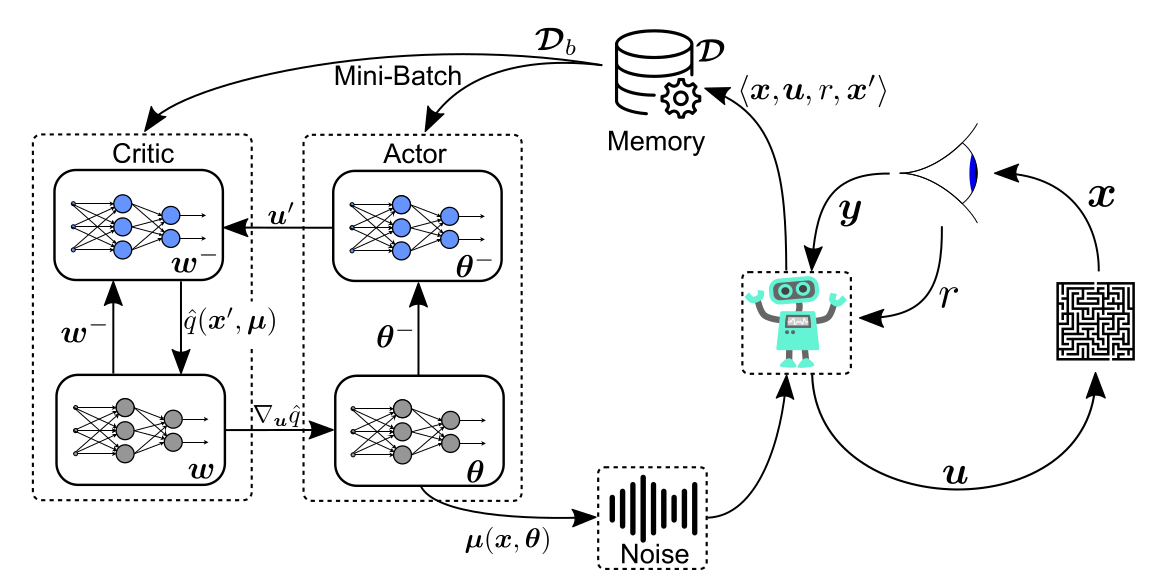
\includegraphics[width=0.75\textwidth]{ddpg.png}
    \caption{DDPG Structure (Source: Oliver Wallscheid's slides on Reinforcement Learning).}
    \end{figure}
\end{frame}

\begin{frame}
  \frametitle{DDPG Algorithm}
    \begin{algorithm}[H]
    \captionsetup{font=scriptsize}
    \caption{Deep Deterministic Policy Gradient}
    \begin{algorithmic}[1]
    \scriptsize
    \STATE Initialize replay buffer $\mathcal{D}$, critic $Q(s, u, w)$ and actor $\mu_\theta(s)$ with random weights $w, \theta$.
    \STATE Initialize target networks $Q'$ and $\mu'$ with weights $w' \leftarrow w$, $\theta' \leftarrow \theta$.
    \FOR{episode = 1, M}
        \STATE Initialize noise process $\mathcal{N}$. Receive initial state $s_1$.
        \FOR{t = 1, T}
            \STATE Select action $u_t = \mu(s_t, \theta) + \mathcal{N}_t$.
            \STATE Execute $u_t$, observe reward $r_t$ and next state $s_{t+1}$.
            \STATE Store transition $(s_t, u_t, r_t, s_{t+1})$ in $\mathcal{D}$.
            \STATE Sample a random mini-batch of $N$ transitions $(s_i, u_i, r_{i}, s_{i+1})$ from $\mathcal{D}$.
            \STATE Set target $y_i = r_i + \gamma Q'(s_{i+1}, \mu'(s_{i+1}, \theta'), w')$.
            \STATE Update critic by minimizing the loss: $L = \frac{1}{N} \sum_i (y_i - Q(s_i, u_i, w))^2$.
            \STATE Update the actor policy using the sampled policy gradient:
            \[ \nabla_\theta J \approx \frac{1}{N} \sum_i \nabla_\theta \mu(s_i, \theta) \nabla_u Q(s_i, u, w)|_{u=\mu(s_i, \theta)} \]
            \STATE Update the target networks:
            \begin{align*}
                w' &\leftarrow \tau w + (1-\tau) w' \\
                \theta' &\leftarrow \tau \theta + (1-\tau) \theta'
            \end{align*}
        \ENDFOR
    \ENDFOR
    \end{algorithmic}
    \end{algorithm}
\end{frame}

%----------------------------------------------------------------------------------------
%	SECTION 4: LIMITATIONS OF DDPG
%----------------------------------------------------------------------------------------

\section{Limitations of DDPG}

\begin{frame}
  \frametitle{Problem 1: Overestimation Bias}
    \begin{itemize}
        \item \textbf{Q-Learning (Recap):} Maximization step in target calculation leads to systematic overestimation bias if initial value estimates are noisy.
        \item \textbf{Does this happen in Actor-Critic?} Yes!
        \begin{itemize}
            \item Function Approximation Error: Neural network critics $Q_w(s,a)$ inevitably have errors.
            \item Policy Updates Interact with Error: If $Q_w$ has positive errors in some regions, the actor might exploit these errors, leading to suboptimal policies that work with the flawed critic.
        \end{itemize}
    \end{itemize}

    \begin{figure}
        \centering
        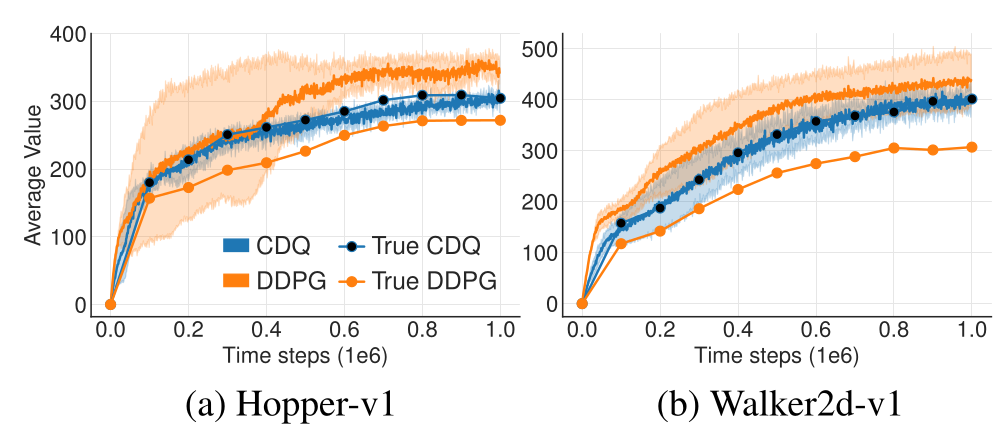
\includegraphics[width=0.5\textwidth]{ddpg-overestimation.png}
        \caption{DDPG often overestimates Q-values compared to true Monte Carlo returns \cite{fujimoto2018addressingfunctionapproximationerror}.}
    \end{figure}
\end{frame}

\begin{frame}
  \frametitle{Problem 2: High Variance from TD Errors}
    \begin{itemize}
        \item Bellman equation is rarely satisfied due to functional approximation. There's always some residual TD error $\delta(s, u)$. This error accumulates over time during bootstrapping.
        \begin{align*}
         Q_w(s_t, u_t) &= r_t + \gamma \mathbb{E}_{s_{t+1}} [Q_w(s_{t+1}, u_{t+1})] - \delta_t \\
         &= \mathbb{E}_\pi \left[ \sum_{k=t}^T \gamma^{k-t} (r_k - \delta_k) \right]
        \end{align*}
        \item The variance of the Q-estimate $Q_w$ depends on the variance of future rewards \textit{and} the variance of future TD errors. High variance would lead to noisy actor gradients and unstable policy updates.
        \item Target networks help by slowing down changes in the target value, reducing the error introduced at each step, but variance can still accumulate.
        \item Frequent policy updates can exacerbate this by constantly changing the ``true'' value target $Q^\pi$, making it harder for the critic to track.
    \end{itemize}
\end{frame}

\begin{frame}
  \frametitle{Problem 2: High Variance from TD Errors}
     \begin{figure}
        \centering
        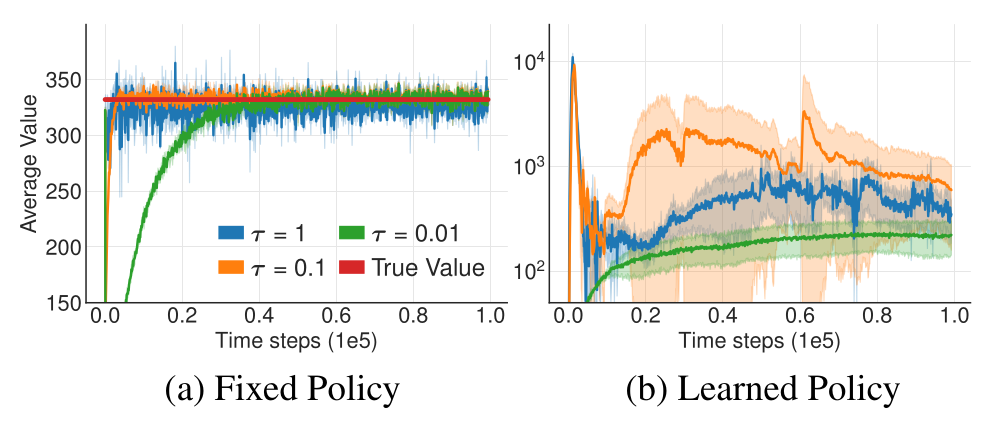
\includegraphics[width=0.6\textwidth]{ddpg-variance.png}
        \caption{Frequent policy and target updates (high value of $\tau$) can increase instability of the estimated value \cite{fujimoto2018addressingfunctionapproximationerror}.}.
    \end{figure}
\end{frame}

%----------------------------------------------------------------------------------------
%	SECTION 5: Twin Delayed DDPG (TD3)
%----------------------------------------------------------------------------------------

\section{Twin Delayed DDPG (TD3)}
\renewcommand{\pageauthor}{Vikaskumar Kalsariya}

\begin{frame}
  \frametitle{TD3: Addressing DDPG's Flaws}
    \textbf{Goal:} Improve DDPG by specifically targeting overestimation bias and high variance.

    \textbf{Three Key Modifications:}
    \begin{enumerate}
        \item \textbf{Clipped Double Q-Learning:} Mitigate actor exploitation of critic errors (address overestimation).
        \item \textbf{Delayed Policy Updates:} Update policy less frequently than critic (reduce variance, stabilize targets).
        \item \textbf{Target Policy Smoothing:} Regularize critic by smoothing Q-estimates w.r.t. actions (reduce variance, prevent sharp peaks).
    \end{enumerate}
\end{frame}

\begin{frame}
  \frametitle{Modification 1: Clipped Double Q-Learning}
    \begin{itemize}
        \item Problem: Standard target network update in DDPG ($y = r + \gamma Q'(s', \mu'(s', \theta'))$) can still overestimate. Double DQN idea (using current policy $\mu$ with target critic $Q'$) is ineffective because $\mu$ and $\mu'$ are too similar.
        \item \textbf{TD3 Approach:}
        \begin{itemize}
            \item Learn \textbf{two} independent critic networks $Q_{w_1}, Q_{w_2}$, along with their target networks $Q'_{w'_1}, Q'_{w'_2}$.
            \item When computing the TD target $y$, use the minimum of the two target critic values:
            \begin{equation*}
            y = r + \gamma \min_{i=1,2} Q'_{w'_i}(s', \tilde{a})
            \end{equation*}
            \item Both critics $Q_{w_1}, Q_{w_2}$ are updated towards this same target $y$.
        \end{itemize}
        \item \textbf{Why?}
        \begin{itemize}
            \item One critic might overestimate, but it's less likely both overestimate identically.
            \item Helps select actions with lower variance Q-value estimates (minimum of two random variables is lower if variance is high).
        \end{itemize}
    \end{itemize}
\end{frame}

\begin{frame}
  \frametitle{Modification 2: Target Policy Smoothing}
    \begin{itemize}
        \item Problem: Deterministic policies $\mu$ can overfit to narrow peaks in the value estimate $Q_w$. Small errors in $Q_w$ can lead to large errors in the target $y$.

        \item \textbf{TD3 Approach:} Smooth the target value calculation \textit{before} evaluating the target critics.
        \begin{itemize}
            \item Compute target action with noise:
            \begin{align*}
            \tilde{a} &= \mu'(s', \theta') + \epsilon \\
            \epsilon &\sim \text{clip}(\mathcal{N}(0, \sigma^2), -c, c)
            \end{align*}
            \item Use this noisy action $\tilde{a}$ in the Clipped Double Q target:
             \begin{equation*}
            y = r + \gamma \min_{i=1,2} Q'_{w'_i}(s', \tilde{a})
            \end{equation*}
        \end{itemize}

        \item \textbf{Why?}
        \begin{itemize}
            \item This allows our deterministic policy to explore more states as well.
            \item Forces the Q-function to be smoother in the action dimension around the policy's actions.
        \end{itemize}
    \end{itemize}
\end{frame}

\begin{frame}
  \frametitle{Modification 3: Delayed Policy Updates}
    \begin{itemize}
        \item Problem: Actor (policy) and Critic (value) can interact poorly. If the Q-estimate is temporarily inaccurate, updating the policy based on it can lead the policy astray. This bad policy then generates poor data, making it harder for the critic to improve. Feedback loop.

        \item \textbf{TD3 Approach:} Update the policy (actor) and target networks less frequently than the value (critic) networks.
        \begin{itemize}
            \item Update critic networks ($Q_{w_1}, Q_{w_2}$) at every step.
            \item Update actor network ($\mu_\theta$) and target networks ($Q'_{w'_1}, Q'_{w'_2}, \mu'_{\theta'}$) only every $d$ critic updates (e.g., $d=2$).
        \end{itemize}

        \item \textbf{Why?}
        \begin{itemize}
            \item Allows the critic(s) more time to converge to a better value estimate based on a relatively stable policy before the policy itself is updated.
            \item Prioritizes reducing value error before updating the policy.
            \item Leads to higher quality policy updates and overall more stable learning. Reduces variance propagation.
        \end{itemize}
    \end{itemize}
\end{frame}

\begin{frame}
  \frametitle{TD3 Algorithm Summary}
    \begin{algorithm}[H]
    \captionsetup{font=scriptsize}
    \caption{Twin Delayed Deep Deterministic Policy Gradient}
    \begin{algorithmic}[1]
    \scriptsize
    \STATE Initialize critic networks $Q_{w_1}, Q_{w_2}$, actor network $\mu_{\theta}$.
    \STATE Initialize target networks $w'_1 \leftarrow w_1, w'_2 \leftarrow w_2, \theta' \leftarrow \theta$.
    \STATE Initialize replay buffer $\mathcal{D}$.
    \FOR{t = 1, T}
        \STATE Select action with exploration noise: $u_t = \mu(s_t, \theta) + \epsilon$, $\epsilon \sim \mathcal{N}(0, \sigma_{explore})$.
        \STATE Execute $u_t$, observe $r_{t+1}, s_{t+1}$. Store $(s_t, u_t, r_{t+1}, s_{t+1})$ in $\mathcal{D}$.
        \STATE Sample mini-batch of $N$ transitions $(s, u, r, s')$ from $\mathcal{D}$.
        \STATE Compute target action with noise: $\tilde{a} \leftarrow \mu'(s', \theta') + \epsilon'$, $\epsilon' \sim \text{clip}(\mathcal{N}(0, \sigma_{target}), -c, c)$. Clip $\tilde{a}$ to valid action range.
        \STATE Compute target Q value: $y \leftarrow r + \gamma \min_{i=1,2} Q'_{w'_i}(s', \tilde{a})$. \COMMENT{Clipped Double Q + Target Smoothing}
        \STATE Update critics $Q_{w_1}, Q_{w_2}$ using gradient descent on $\frac{1}{N}\sum (y - Q_{w_i}(s, u))^2$.
        \IF{t mod d == 0}
            \STATE Update actor $\mu_\theta$ using the deterministic policy gradient w.r.t. $Q_{w_1}$:
            \[ \nabla_\theta J \approx \frac{1}{N} \sum \nabla_\theta \mu_\theta(s) \nabla_u Q_{w_1}(s, u)|_{u=\mu_\theta(s)} \]
            \STATE Update target networks using soft updates ($\tau \ll 1$):
            \begin{align*}
                w'_i &\leftarrow \tau w_i + (1-\tau) w'_i \quad \text{for } i=1,2 \\
                \theta' &\leftarrow \tau \theta + (1-\tau) \theta'
            \end{align*}
        \ENDIF
    \ENDFOR
    \end{algorithmic}
    \end{algorithm}
\end{frame}

\begin{frame}
  \frametitle{TD3 Convergence Sketch (Tabular Clipped Double Q)}
    \begin{itemize}
        \item \textbf{Foundation:} Leverages standard stochastic approximation theory (conditions ensuring iterative updates converge).

        \item \textbf{Goal:} Show the Q-value error $\Delta_t = Q_t - Q^*$ converges towards 0.

        \item \textbf{Proof Outline:}
        \begin{enumerate}
            \item Show the update rule fits the stochastic approximation framework (requires specific learning rate conditions).
            \item Prove that the difference between the two critic estimates ($\Delta^{BA} = Q^B - Q^A$) converges to zero. 
            \item The update step pulls both $Q^A(s,a)$ and $Q^B(s,a)$ towards this common target $y$.
            \item Argue that once $Q^A \approx Q^B$, the update resembles standard Q-learning (known to converge under tabular conditions).
        \end{enumerate}
    \end{itemize}
\end{frame}

%----------------------------------------------------------------------------------------
%	SECTION 6: Hindsight Experience Replay (HER)
%----------------------------------------------------------------------------------------

\section{Hindsight Experience Replay (HER)}

\begin{frame}
  \frametitle{Motivation: The Sparse Reward Problem}
    \begin{itemize}
        \item Many real-world tasks (especially robotics) have sparse rewards: reward is 0 until the task is fully completed, then maybe 1.
        \item Example: Robot arm needs to push a block to location G. Reward is 0 unless the block is exactly at G.
        \item Standard RL algorithms (DQN, DDPG, TD3) struggle immensely with sparse rewards. Why?
        \begin{itemize}
            \item Learning signal is almost always 0.
            \item Extremely unlikely to achieve the goal by random exploration initially.
            \item Agent gets no feedback on whether it's making progress.
        \end{itemize}

        \item Traditional Solution: Reward Shaping \cite{10.5555/645528.657613}.
            \begin{itemize}
                \item Manually design dense reward functions (e.g., reward proportional to negative distance to goal).
                \item Requires significant domain expertise and careful tuning.
            \end{itemize}

        \item \textbf{Question:} Can we learn efficiently from sparse (binary) rewards without manual shaping?
    \end{itemize}
\end{frame}

\begin{frame}
  \frametitle{HER: The Core Idea - Learning from Failure}
  \begin{itemize}
    \item Consider an episode where the agent tried to achieve goal $g$, took actions $a_1, \dots, a_T$, visited states $s_1, \dots, s_T$, and failed (never received positive reward).
    \item Standard RL: This trajectory provides little learning signal (all rewards were 0 or negative).

    \item \textbf{HER Insight:} The trajectory still contains useful information about how to reach the states that \textit{were} visited.
    \item \textbf{Hindsight Replay Mechanism:}
        \begin{enumerate}
            \item Execute an episode with the original goal $g$. Store the trajectory $(s_0, a_0, r_0, s_1, ..., s_T)$.
            \item For each transition $(s_t, a_t, r_t, s_{t+1})$ in the trajectory:
                \begin{itemize}
                    \item Store it in the replay buffer $\mathcal{D}$ with the original goal $g$.
                    \item Sample a set of \textit{additional} goals $\mathcal{G}'$ based on states achieved \textit{in the same episode}.
                    \item For each additional goal $g' \in \mathcal{G}'$:
                        \begin{itemize}
                            \item Calculate a new reward $r'_t = r(s_t, a_t, g')$.
                            \item Store the modified transition $(s_t, a_t, r'_t, s_{t+1})$ in $\mathcal{D}$ with the hindsight goal $g'$.
                        \end{itemize}
                \end{itemize}
        \end{enumerate}
    \item The agent learns how to achieve goals it accidentally encountered, even when failing at the original task.
  \end{itemize}
\end{frame}

\begin{frame}
  \frametitle{HER Requirements: Multi-Goal RL}
    \begin{itemize}
        \item HER naturally operates in a multi-goal setting.
        \item We need policies and value functions that are conditioned on the goal $g$:
        \begin{itemize}
            \item Policy: $\pi(s, g)$ or $\mu(s, g)$
            \item Q-function: $Q(s, a, g)$
        \end{itemize}
        \item The reward function $r(s, a, g)$ must be computable for any state-action pair $(s, a)$ and \textit{any potential goal} $g$.
            \begin{itemize}
                \item For sparse binary rewards: $r(s, a, g') = 0$ if $s_{t+1}$ satisfies goal $g'$, and $-1$ otherwise. (Or 1 and 0).
            \end{itemize}

        \item Need a mapping $m: \mathcal{S} \to \mathcal{G}$ that extracts the achieved goal aspect from a state $s$.
            \begin{itemize}
                \item Example: If states $s$ include object position $s_{obj}$ and goals $g$ are desired object positions, then $m(s) = s_{obj}$.
            \end{itemize}
    \end{itemize}
\end{frame}

\begin{frame}
  \frametitle{HER Algorithm}
    \begin{algorithm}[H]
    \captionsetup{font=small}
    \caption{Hindsight Experience Replay}
    \begin{algorithmic}[1]
    \scriptsize
    \REQUIRE Off-policy RL algorithm $\mathcal{A}$ (e.g., DDPG, TD3).
    \REQUIRE Reward function $r: \mathcal{S} \times \mathcal{A} \times \mathcal{G} \to \mathbb{R}$.
    \REQUIRE Strategy $\mathcal{S}$ for sampling hindsight goals.
    \REQUIRE Hindsight-to-original goal ratio $k$.
    \STATE Initialize algorithm $\mathcal{A}$, replay buffer $\mathcal{R}$.
    \FOR{episode = 1 to M}
        \STATE Sample initial state $s_0$ and goal $g$. Store episode trajectory $\tau = (s_0, a_0, ..., s_T)$.
        \FOR{$t = 0$ to $T-1$}
            \STATE Compute reward $r_t = r(s_t, a_t, g)$.
            \STATE Store original transition $(s_t || g, a_t, r_t, s_{t+1} || g)$ in $\mathcal{R}$. \COMMENT{Store with original goal}
            \STATE Sample set of additional goals $\mathcal{G}' = \mathcal{S}(\text{episode } \tau)$.
            \FOR{$g' \in \mathcal{G}'$}
                 \STATE Compute hindsight reward $r'_t = r(s_t, a_t, g')$.
                 \STATE Store hindsight transition $(s_t || g', a_t, r'_t, s_{t+1} || g')$ in $\mathcal{R}$. \COMMENT{Store with hindsight goal}
            \ENDFOR
        \ENDFOR
        \FOR{optimization step = 1 to N}
             \STATE Sample mini-batch $B$ from $\mathcal{R}$.
             \STATE Perform optimization step using $\mathcal{A}$ on $B$.
        \ENDFOR
    \ENDFOR
    \end{algorithmic}
    \end{algorithm}
\end{frame}

\begin{frame}
  \frametitle{HER: Hindsight Goal Sampling Strategies}
    How to choose the additional goals $g'$ for replay from an episode $(s_0, ..., s_T)$?
    \begin{description}
        \item[final] Sample only the goal corresponding to the final state: $g' = m(s_T)$. Simplest version.

        \item[future] For each transition $(s_t, a_t, s_{t+1})$, sample $k$ states $s_{t'}$ from the \textit{rest of the trajectory} ($t' > t$). Use $g' = m(s_{t'})$ as hindsight goals. Rationale: These are goals achieved ``soon'' after the transition. $k=4,8$ often performs best.

        \item[episode] For each transition $(s_t, a_t, s_{t+1})$, sample $k$ states $s_{t'}$ randomly from the \textit{entire episode} ($0 \le t' \le T$). Use $g' = m(s_{t'})$.

        \item[random] Sample $k$ states $s_{t'}$ encountered previously across \textit{all episodes} stored in the replay buffer. Use $g' = m(s_{t'})$.
    \end{description}
\end{frame}


\begin{frame}
  \frametitle{HER: Hindsight Goal Sampling Strategies}
    \begin{figure}
        \centering
        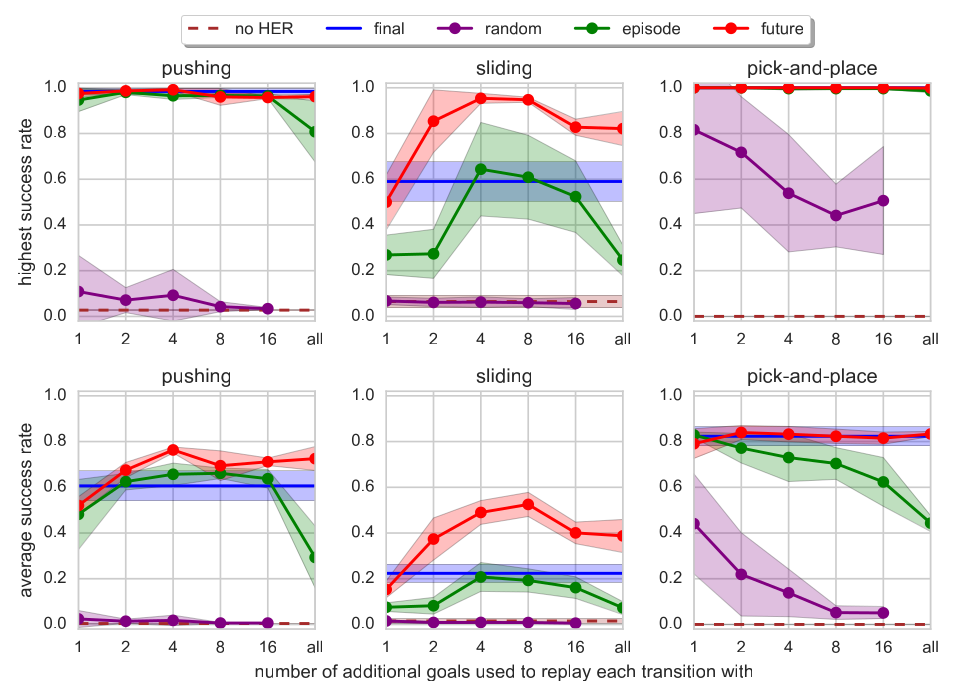
\includegraphics[width=0.5\textwidth]{her-strategies.png}
        \caption{Comparison of HER strategies \cite{andrychowicz2018hindsightexperiencereplay}. The hyperparameter $k$ controls the ratio of HER transitions to original transitions.}
    \end{figure}
\end{frame}

%----------------------------------------------------------------------------------------
%	SECTION 7: RESULTS & SUMMARY
%----------------------------------------------------------------------------------------

\section{Results \& Summary}

\begin{frame}
  \frametitle{TD3 Performance}
    \begin{figure}
        \centering
        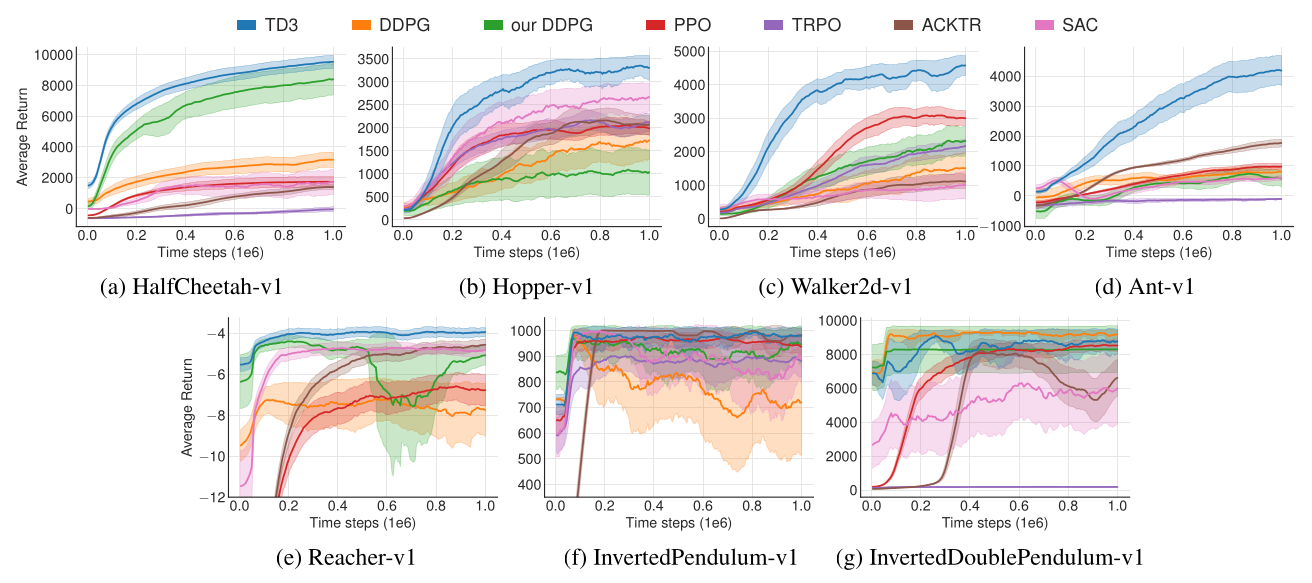
\includegraphics[width=0.8\textwidth]{td3-performance.png}
        \caption{TD3 performance compared to DDPG, PPO, ACKTR, TRPO, SAC on OpenAI Gym MuJoCo tasks \cite{fujimoto2018addressingfunctionapproximationerror}. TD3 generally achieves state-of-the-art performance and stability.}
    \end{figure}
\end{frame}

\begin{frame}
  \frametitle{HER Performance}
    \begin{columns}[T] % Align columns at the top
        \begin{column}{0.2\textwidth}
            \textbf{Bit Flipping}
            \begin{figure}
                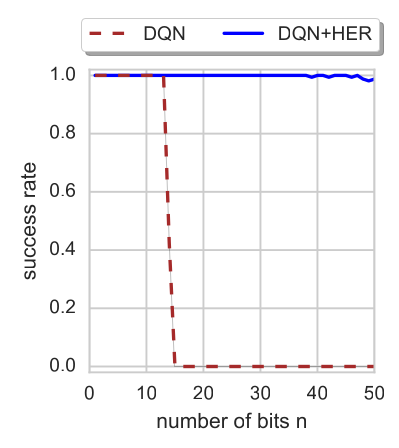
\includegraphics[width=\textwidth]{her-bitflip.png}
                \caption{DQN vs DQN+HER on n-bit flipping. HER enables learning for large n \cite{andrychowicz2018hindsightexperiencereplay}.}
            \end{figure}
        \end{column}
        \begin{column}{0.7\textwidth}
            \textbf{Robotics Tasks (Sparse Reward)}
             \begin{figure}
                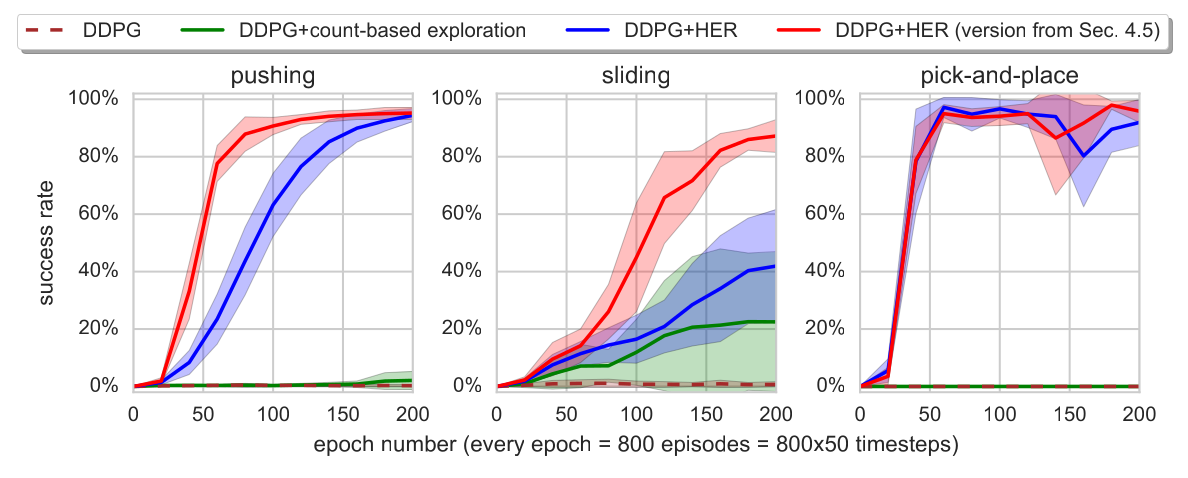
\includegraphics[width=\textwidth]{her-learning-curve.png}
                \caption{DDPG+HER vs DDPG and DDPG+Counts. HER is crucial for learning complex manipulation with sparse rewards \cite{andrychowicz2018hindsightexperiencereplay}.}
            \end{figure}
        \end{column}
    \end{columns}
    \vspace{1em}
\end{frame}

\begin{frame}
  \frametitle{Summary: What We Learned Today}
    \begin{itemize}
        \item \textbf{Deterministic Policy Gradient (DPG):} An alternative to stochastic policy gradients, suitable for continuous actions, enabling off-policy learning. Requires external exploration.

        \item \textbf{Deep DPG (DDPG):} Combines DPG with DQN techniques (replay buffer, target networks) for deep RL in continuous control. Often suffers from Q-value overestimation and high variance.

        \item \textbf{Twin Delayed DDPG (TD3):} Addresses DDPG's issues via Clipped Double Q-Learning, Delayed Policy Updates, and Target Policy Smoothing for improved stability and performance.
        \item \textbf{Hindsight Experience Replay (HER):} A technique for learning with sparse rewards by replaying trajectories with achieved goals as desired goals. Compatible with off-policy algorithms like DDPG/TD3. Avoids reward shaping.
    \end{itemize}
\end{frame}

%----------------------------------------------------------------------------------------
%	SECTION 8: POTENTIAL RESEARCH DIRECTIONS
%----------------------------------------------------------------------------------------

\section{Potential Research Directions}

\begin{frame}
  \frametitle{Extending DPG/TD3/HER: Future Ideas}

    \begin{itemize}
        \item \textbf{Synergy between TD3 and HER:}
            \begin{itemize}
                \item How do TD3's stability improvements interact with HER's relabeling? Does TD3 reduce potential noise introduced by HER?
                \item Can the TD3 components (twin critics, smoothing, delay) be adapted specifically for goal-conditioned settings used with HER?
            \end{itemize}

        \item \textbf{Sample Efficiency \& Model Use:}
            \begin{itemize}
                \item Can HER be integrated with model-based RL to generate imagined trajectories that are then relabeled with hindsight goals?
                \item More efficient HER sampling: Smarter selection of hindsight goals beyond 'future'? Prioritizing hindsight transitions?
            \end{itemize}
    \end{itemize}
\end{frame}

\begin{frame}
  \frametitle{Extending DPG/TD3/HER: Future Ideas (Cont.)}

    \begin{itemize}
         \item \textbf{Theoretical Understanding:}
            \begin{itemize}
                \item Convergence analysis for DDPG/TD3 combined with HER, especially with function approximation.
                \item Analysis of the implicit curriculum generated by different HER sampling strategies.
            \end{itemize}

        \item \textbf{Beyond Simple Goal Achievement:}
            \begin{itemize}
                 \item Using HER for tasks with more complex success criteria than reaching a specific state/configuration?
                 \item Hierarchical RL where HER operates at different levels of abstraction? Relabeling sub-goals?
            \end{itemize}

        \item \textbf{Multi-Agent HER:}
             \begin{itemize}
                \item Applying HER in multi-agent settings. How to define and relabel joint goals or individual goals based on collective outcomes?
             \end{itemize}
    \end{itemize}
\end{frame}

%----------------------------------------------------------------------------------------
%   REFERENCES
%----------------------------------------------------------------------------------------

\section{}
\renewcommand{\pageauthor}{}
\begin{frame}[plain, allowframebreaks]{References}
   \printbibliography[heading=none]
\end{frame}

\begin{frame}
    \centering
    \Huge Thank You!

    \vspace{1cm}
    \normalsize Questions?
\end{frame}

\end{document}
